\documentclass[preprint,12pt]{elsarticle}

\usepackage{amsmath,amssymb}
\usepackage{booktabs}
\usepackage{array}
\usepackage{tabularx}
\usepackage{enumitem}
\usepackage{hyperref}
\usepackage{multirow}
\usepackage{graphicx}
\biboptions{numbers,sort&compress}

\journal{ISPRS Journal of Photogrammetry and Remote Sensing}

\begin{document}

\begin{frontmatter}

\title{Risk-Guided Selective Refinement for UAV Image-Based Geometry Reconstruction}

\author{Anonymous Author}

\begin{abstract}
This paper investigates a selective-refinement strategy for UAV image-based geometry reconstruction under limited computation budget. Instead of refining an entire image sequence with a heavy model, the proposed method first applies DUSt3R to obtain a coarse scene-wide geometric prior, then estimates a frame-level reconstruction risk score, and finally refines only the highest-risk frames with MASt3R. The resulting pipeline is evaluated on two real UAV datasets, namely Dronescapes and ODMData. On Dronescapes, the proposed method achieves an RMSE of 447.81 compared with 447.94 for DUSt3R, while refining only 25\% of the frames. On ODMData, evaluated through projected depth maps obtained from a saved COLMAP/OpenMVS reconstruction, MASt3R achieves the lowest RMSE of 0.1801, while the proposed method reaches 0.2188 while refining only 6.9\% of the frames. The experiments show that risk-guided selective refinement consistently improves a coarse full-pass baseline on Dronescapes and remains competitive on ODMData while refining substantially fewer frames than a full-pass solution. These findings indicate that selective refinement is a viable direction for computation-aware UAV reconstruction, although the current formulation does not yet dominate full-pass MASt3R in absolute accuracy. The implementation used in this study is publicly available at \url{https://github.com/duy12i1i7/GEO}.
\end{abstract}

\begin{keyword}
UAV reconstruction \sep selective refinement \sep DUSt3R \sep MASt3R \sep Dronescapes \sep ODMData
\end{keyword}

\end{frontmatter}

\section{Introduction}

Image-based UAV reconstruction has evolved from classical photogrammetry and structure-from-motion (SfM) pipelines into a broader ecosystem that also includes multi-view stereo (MVS), dense matching, and learning-based geometric inference \citep{Colomina2014Unmanned,Jiang2017Efficient,Jiang2020Efficient,Schonberger2016SfM,Liu2023Deep,Liao2024High}. For many practical deployments, the main question is no longer whether a scene can be reconstructed at all, but whether it can be reconstructed under a constrained compute budget.

Classical pipelines such as COLMAP followed by downstream MVS remain strong baselines for geometry quality, but they are often expensive in both setup and runtime \citep{Schonberger2016SfM}. Recent pointmap-based models such as DUSt3R and MASt3R make dense geometric reasoning much easier from image collections \citep{Wang2024DUSt3R,Leroy2024MASt3R}, yet full-pass processing over all frames still carries a significant cost. This motivates a simple question: should all frames be refined equally?

This paper studies a selective alternative. The central hypothesis is that some frames are already sufficiently explained after a coarse scene-wide pass, whereas others remain geometrically risky because of weak overlap, poor texture, or less favorable viewpoint placement. If a system can identify these risky frames and allocate expensive refinement only to them, it may achieve a better quality--cost trade-off than uniform processing.

Based on this idea, we implement and evaluate \textbf{risk-guided hybrid refinement}. The pipeline runs DUSt3R over the full image set, computes a frame-wise reconstruction risk score, applies MASt3R only to the top-ranked frames, and merges coarse and refined predictions into the final output. The method is benchmarked on two real UAV datasets, Dronescapes \citep{DronescapesDataset} and ODMData \citep{ODMDataBenchmarks}.

The contributions of the paper are:
\begin{enumerate}[leftmargin=1.5em]
  \item a frame-level risk-guided selective refinement formulation for UAV geometry reconstruction;
  \item a practical hybrid pipeline that combines DUSt3R coarse inference with MASt3R refinement;
  \item a two-dataset empirical study on Dronescapes and ODMData;
  \item an analysis showing that selective refinement improves over a coarse full-pass baseline while approaching a stronger full-pass solution with fewer refined frames.
\end{enumerate}

\section{Related work}

\subsection{UAV photogrammetry and image-based reconstruction}

UAV photogrammetry has become a major platform for mapping and 3D reconstruction \citep{Colomina2014Unmanned}. Efficient SfM for large or oblique UAV image collections has been widely studied, with improvements in image pair selection, graph design, and scalable merging \citep{Jiang2017Efficient,Jiang2020Efficient,Jiang2022Leveraging,Jiang2022Parallel,Jiang2024Efficient}. In parallel, dense multi-view methods, including deep learning based variants, have improved completeness and robustness for urban-scale reconstruction \citep{Liu2023Deep,Liao2024High}.

These pipelines typically process all frames in a relatively uniform manner. That assumption is natural for standard offline photogrammetry, but it leaves open the question of whether every frame really deserves the same refinement budget.

\subsection{Learning-based geometric reconstruction}

DUSt3R reformulates geometric reconstruction through direct pointmap prediction and thereby simplifies several 3D vision tasks from image collections \citep{Wang2024DUSt3R}. MASt3R extends this direction by improving matching robustness and geometric consistency through 3D-grounded image matching \citep{Leroy2024MASt3R}. Evaluations on aerial photogrammetric blocks suggest that these methods are particularly promising in sparse and difficult reconstruction regimes \citep{Wu2025AerialBlocks}.

However, learning-based full-pass inference does not solve the question of budget allocation by itself. Even when inference is easier than a classical MVS pipeline, refining every frame remains costly.

\subsection{Confidence, uncertainty and selective processing}

Confidence-aware dense geometry estimation has long been recognized as important for robust reconstruction \citep{Li2020Confidence}. Related ideas also appear in SLAM and localization pipelines, where uncertainty helps decide how observations should influence the evolving model \citep{Campos2021ORB,Qin2018VINS,Wang2024Benchmarking}. The present work adopts the same spirit but focuses specifically on frame-level selective refinement for UAV reconstruction.

\section{Method}

\subsection{Problem formulation}

Given an image set $\mathcal{I}=\{I_i\}_{i=1}^{N}$, the objective is to reconstruct scene geometry while reducing unnecessary expensive refinement. Let $\mathcal{S}\subseteq \mathcal{I}$ be the subset selected for heavy refinement. The design goal can be written conceptually as
\[
\min_{\mathcal{S}} \; \mathcal{L}_{geo}(\hat{\mathcal{D}}(\mathcal{I},\mathcal{S})) + \lambda \mathcal{C}(\mathcal{S}),
\]
where $\hat{\mathcal{D}}$ is the final merged reconstruction and $\mathcal{C}(\mathcal{S})$ denotes computation cost.

\subsection{Pipeline}

The proposed pipeline contains four stages.

\textbf{Stage 1: coarse global reconstruction.}
DUSt3R is applied to the full dataset to obtain a scene-wide coarse geometric prior.

\textbf{Stage 2: frame-wise risk estimation.}
For each frame, the system computes a reconstruction risk score from four normalized terms:
\begin{itemize}[leftmargin=1.5em]
  \item \textbf{overlap term} $O_i$, increasing when neighboring frames provide weaker support;
  \item \textbf{texture term} $T_i$, increasing when image texture is weak;
  \item \textbf{depth term} $D_i$, capturing uncertainty in an optional depth prior;
  \item \textbf{view term} $V_i$, reflecting viewpoint disadvantage relative to the sequence center.
\end{itemize}

The current implementation uses
\[
R_i = 0.35 O_i + 0.25 T_i + 0.20 D_i + 0.20 V_i.
\]

Operationally, $O_i$ comes from one minus the average cosine similarity to nearby grayscale frames, $T_i$ from one minus normalized grayscale standard deviation, $D_i$ from the dispersion of valid prior depth values when such a prior exists, and $V_i$ from normalized distance to the temporal sequence center.

\textbf{Stage 3: selective refinement.}
Only the top-$K$ frames with highest $R_i$ are refined by MASt3R. In the reported run, $K=8$.

\textbf{Stage 4: merge.}
Refined predictions overwrite or merge with DUSt3R coarse outputs to produce the final benchmarked result.

\subsection{Interpretation of the contribution}

The contribution is not a new 3D backbone. Instead, it changes the allocation policy: the method treats \textit{where to spend refinement} as the optimization target. In that sense, it reframes UAV reconstruction from ``refine everything equally'' to ``refine selectively under a budget''.

\section{Experimental setup}

\subsection{Datasets}

\textbf{ODMData.}
The benchmark uses the \texttt{mygla} sample from the OpenDroneMap benchmark collection \citep{ODMDataBenchmarks}. The prepared split contains 29 frames in the reported run.

\textbf{Dronescapes.}
The benchmark uses \texttt{test\_set\_annotated\_only} from Dronescapes \citep{DronescapesDataset}, with 32 frames in the reported POC configuration. A practical detail is that the public release used here stores RGB data in \texttt{.npz} form, so the GEO pipeline converts them into \texttt{.png} during export to create a consistent image-depth structure.

\subsection{Compared methods}

The reported benchmark includes:
\begin{enumerate}[leftmargin=1.5em]
  \item \textbf{DUSt3R full-pass} (\texttt{dust3r\_real});
  \item \textbf{MASt3R full-pass} (\texttt{mast3r\_real});
  \item \textbf{risk-guided hybrid refinement} (\texttt{risk\_hybrid\_real}).
\end{enumerate}

Although the broader experimental framework also supports \texttt{COLMAP + OpenMVS}, the reported run is intentionally focused on the comparison between coarse, full-refinement, and selective-refinement learned pipelines.

\subsection{Implementation details}

Table~\ref{tab:implementation-details} summarizes the implementation and hardware configuration.

\begin{table}[t]
\centering
\small
\begin{tabular}{lp{8.2cm}}
\toprule
Setting & Value \\
\midrule
Coarse image size & 224 \\
Refine image size & 384 \\
Batch size & 1 \\
Window size & 2 \\
Top-$K$ refined frames & 8 \\
Risk neighbors & 4 \\
Coarse/refine device & CUDA \\
CPU & Intel Core Ultra 9 285K \\
System memory & 60~GiB RAM \\
GPU & NVIDIA RTX 5000 Ada 32~GiB \\
Operating system & Ubuntu 24.04.4 \\
\bottomrule
\end{tabular}
\caption{Implementation and hardware details of the reported experiment.}
\label{tab:implementation-details}
\end{table}

The implementation and benchmark scripts used in this study are publicly available at \url{https://github.com/duy12i1i7/GEO}.

\section{Results}

\subsection{Dronescapes}

\begin{table}[t]
\centering
\small
\begin{tabular}{lcccc}
\toprule
Method & MAE & RMSE & AbsRel & Selected ratio \\
\midrule
DUSt3R & 345.054 & 447.936 & 0.9905 & 1.00 \\
MASt3R & \textbf{343.628} & \textbf{446.506} & \textbf{0.9858} & 1.00 \\
Risk-hybrid & 344.913 & 447.812 & 0.9900 & 0.25 \\
\bottomrule
\end{tabular}
\caption{Results on \texttt{dronescapes\_poc\_real}.}
\label{tab:dronescapes-isprs}
\end{table}

Table~\ref{tab:dronescapes-isprs} shows that MASt3R full-pass remains the strongest method in absolute depth accuracy. The proposed method improves slightly but consistently over DUSt3R while refining only 25\% of the frames. This supports the selective-refinement hypothesis and suggests that the risk score is able to identify informative frames with non-trivial geometric value.

Importantly, all entries in Table~\ref{tab:dronescapes-isprs} are direct ground-truth evaluation results from the reported server run.

\subsection{ODMData}

\begin{table}[t]
\centering
\small
\begin{tabular}{lcccc}
\toprule
Method & MAE & RMSE & AbsRel & Selected ratio \\
\midrule
DUSt3R & 0.1576 & 0.2184 & 0.0337 & 1.00 \\
MASt3R & \textbf{0.1299} & \textbf{0.1801} & \textbf{0.0274} & 1.00 \\
Risk-hybrid & 0.1584 & 0.2188 & 0.0340 & 0.069 \\
\bottomrule
\end{tabular}
\caption{Results on \texttt{odmdata\_odm\_poc\_mygla\_real} using projected COLMAP/OpenMVS depth maps for relative depth comparison.}
\label{tab:odm-isprs}
\end{table}

On ODMData, MASt3R is the closest learned method to the projected COLMAP/OpenMVS depth reconstruction used in the comparison. The proposed method remains in the same error band as DUSt3R while refining only about 6.9\% of the frames, which is still useful from a budget-allocation perspective. The ODMData table should therefore be read primarily as a relative depth comparison rather than as a substitute for direct ground-truth geometric evaluation.

\section{Qualitative results}

Quantitative metrics alone do not fully reveal how the selective-refinement policy changes the reconstructed geometry. To provide a denser visual comparison, this section organizes the current benchmark outputs into a single three-by-three qualitative summary. The first row compares depth predictions on Dronescapes, the second row compares the corresponding error maps on Dronescapes, and the third row compares depth predictions on ODMData. Taken together, these panels illustrate how the proposed selective-refinement strategy positions itself between a coarse full-pass baseline and a stronger full-pass refinement baseline.

Figure~\ref{fig:qualitative-grid} shows three consistent trends. First, on Dronescapes, MASt3R yields the visually strongest full-pass geometry, which is consistent with the quantitative ordering in Table~\ref{tab:dronescapes-isprs}. Second, the proposed method preserves the same large-scale scene structure while reducing part of the coarse behavior visible in DUSt3R. Third, the ODMData row suggests that selective refinement steers the coarse prediction toward a more refined geometry without requiring heavy refinement on every frame.

\begin{figure}[p]
\centering
\begin{minipage}[t]{0.31\linewidth}
\centering
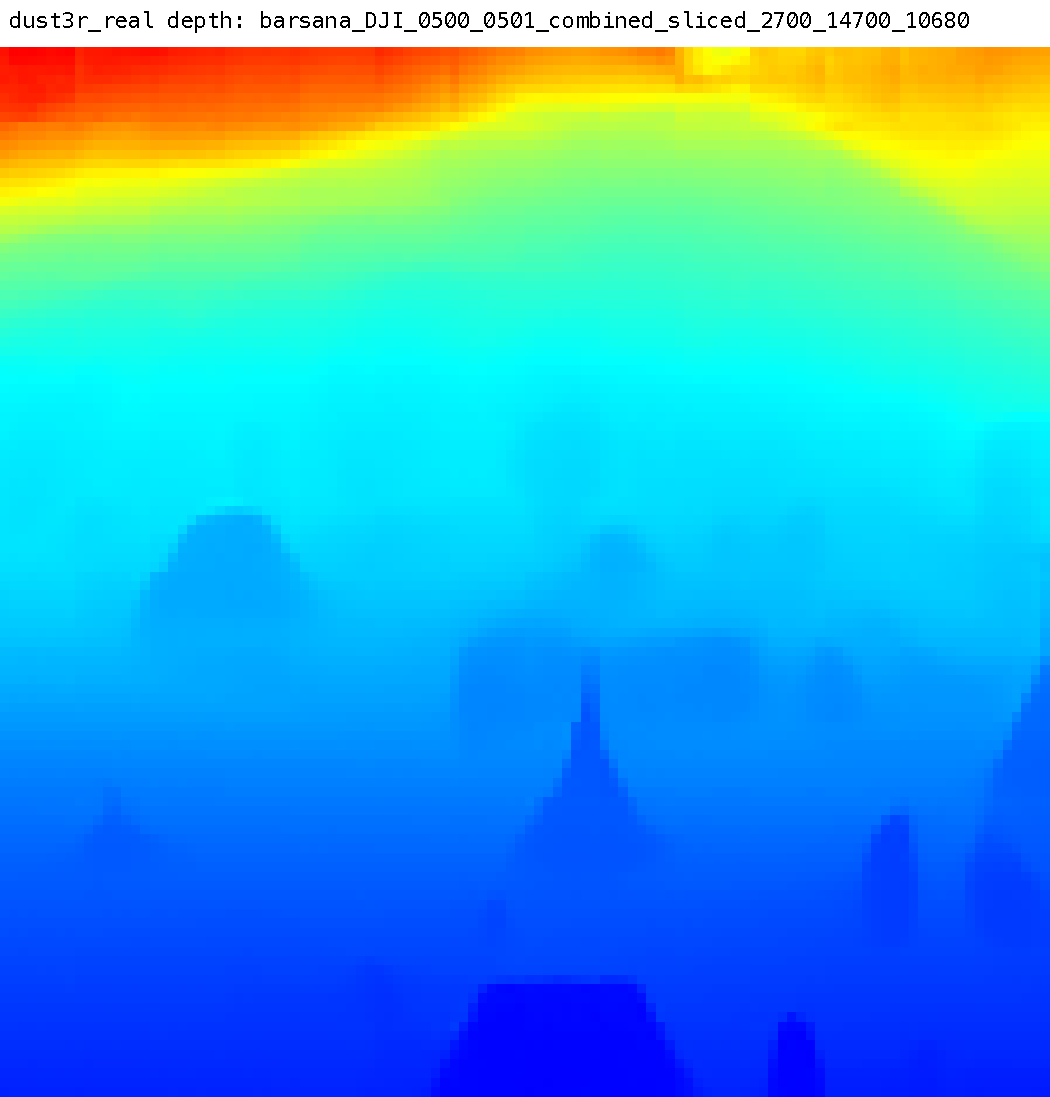
\includegraphics[width=\linewidth]{figures/dronescapes_dust3r_depth.pdf}

\small (a) Dronescapes, DUSt3R depth
\end{minipage}\hfill
\begin{minipage}[t]{0.31\linewidth}
\centering
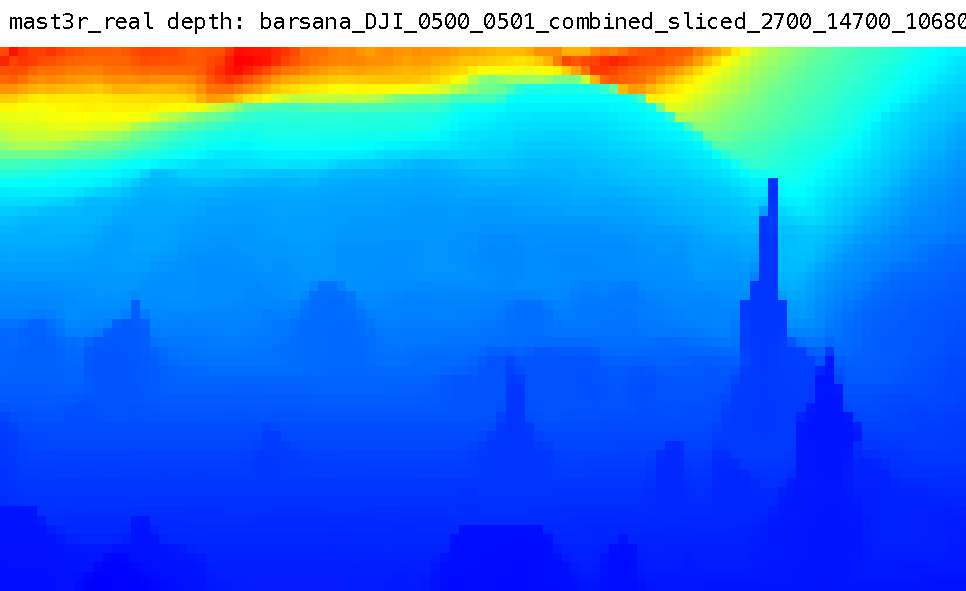
\includegraphics[width=\linewidth]{figures/dronescapes_mast3r_depth.pdf}

\small (b) Dronescapes, MASt3R depth
\end{minipage}\hfill
\begin{minipage}[t]{0.31\linewidth}
\centering
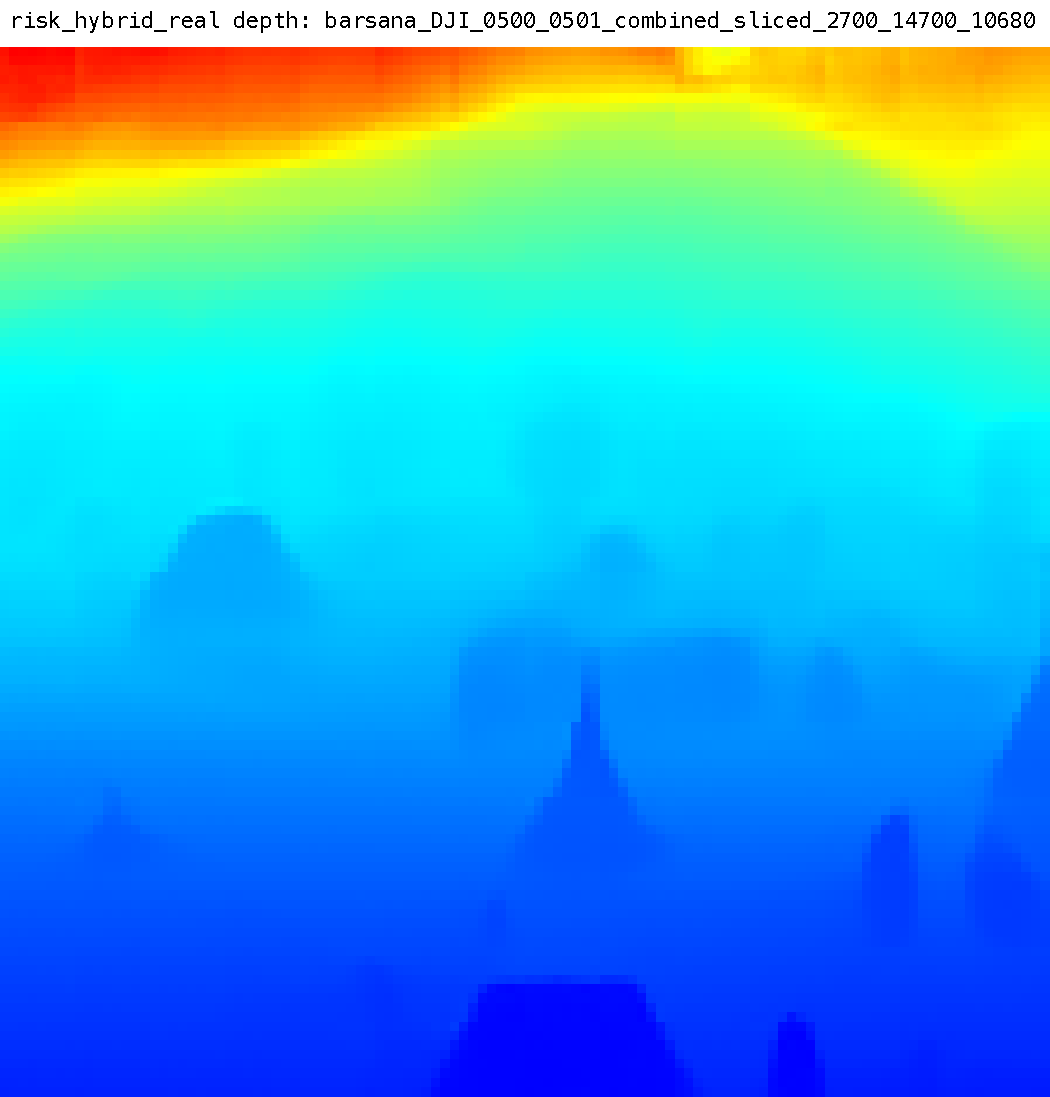
\includegraphics[width=\linewidth]{figures/dronescapes_risk_depth.pdf}

\small (c) Dronescapes, risk-hybrid depth
\end{minipage}

\vspace{0.8em}

\begin{minipage}[t]{0.31\linewidth}
\centering
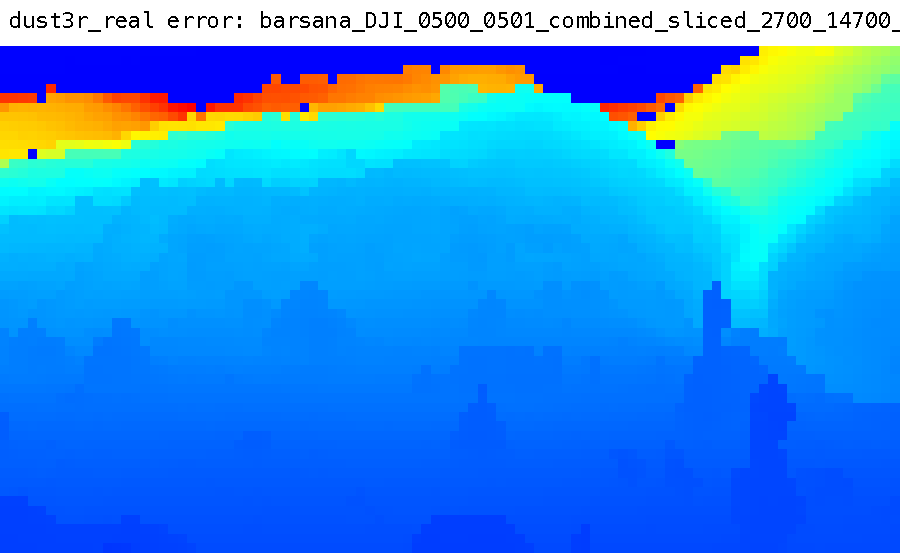
\includegraphics[width=\linewidth]{figures/dronescapes_dust3r_error.pdf}

\small (d) Dronescapes, DUSt3R error
\end{minipage}\hfill
\begin{minipage}[t]{0.31\linewidth}
\centering
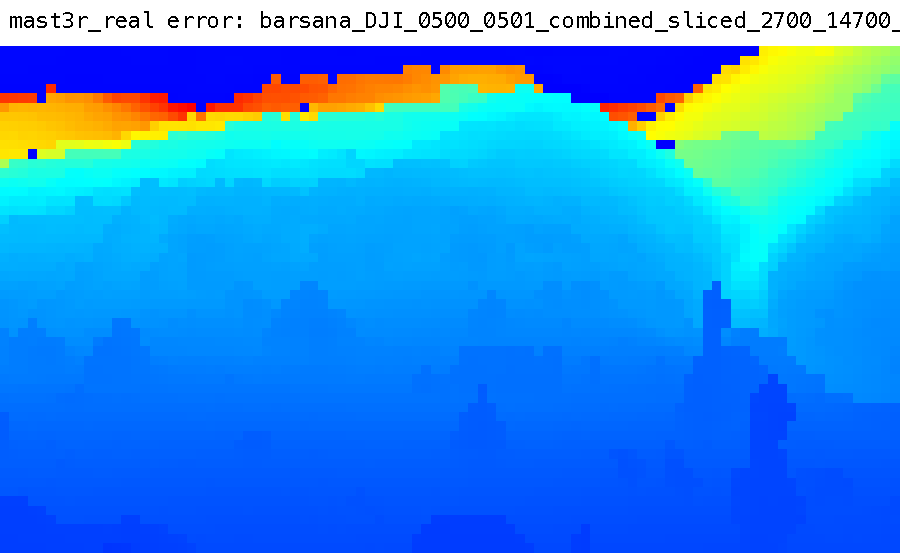
\includegraphics[width=\linewidth]{figures/dronescapes_mast3r_error.pdf}

\small (e) Dronescapes, MASt3R error
\end{minipage}\hfill
\begin{minipage}[t]{0.31\linewidth}
\centering
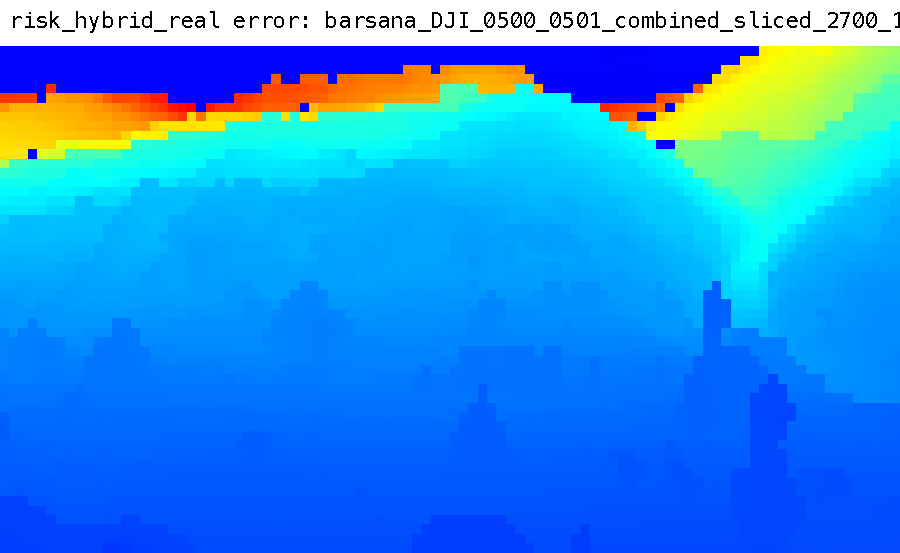
\includegraphics[width=\linewidth]{figures/dronescapes_risk_error.pdf}

\small (f) Dronescapes, risk-hybrid error
\end{minipage}

\vspace{0.8em}

\begin{minipage}[t]{0.31\linewidth}
\centering
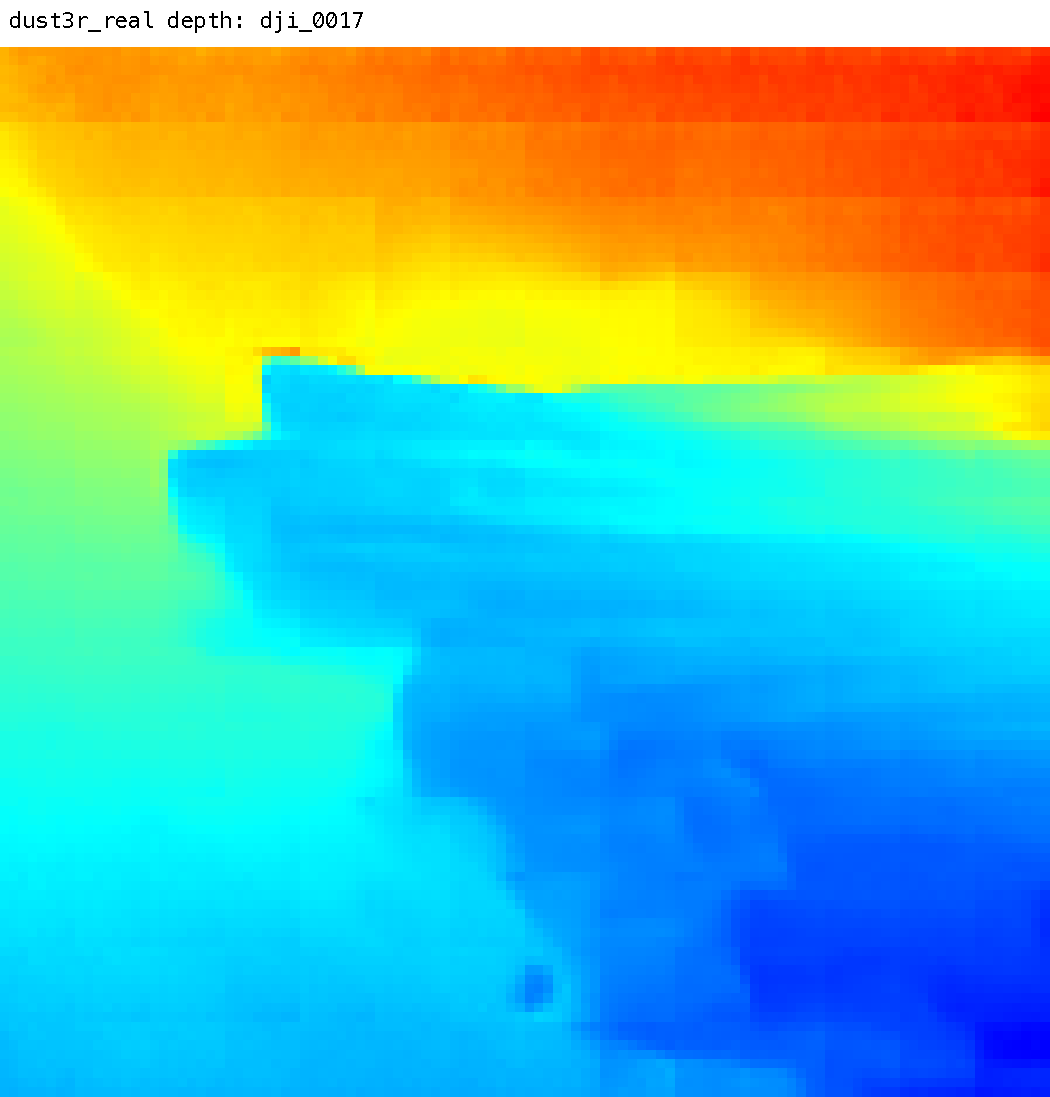
\includegraphics[width=\linewidth]{figures/odmdata_dust3r_depth.pdf}

\small (g) ODMData, DUSt3R depth
\end{minipage}\hfill
\begin{minipage}[t]{0.31\linewidth}
\centering
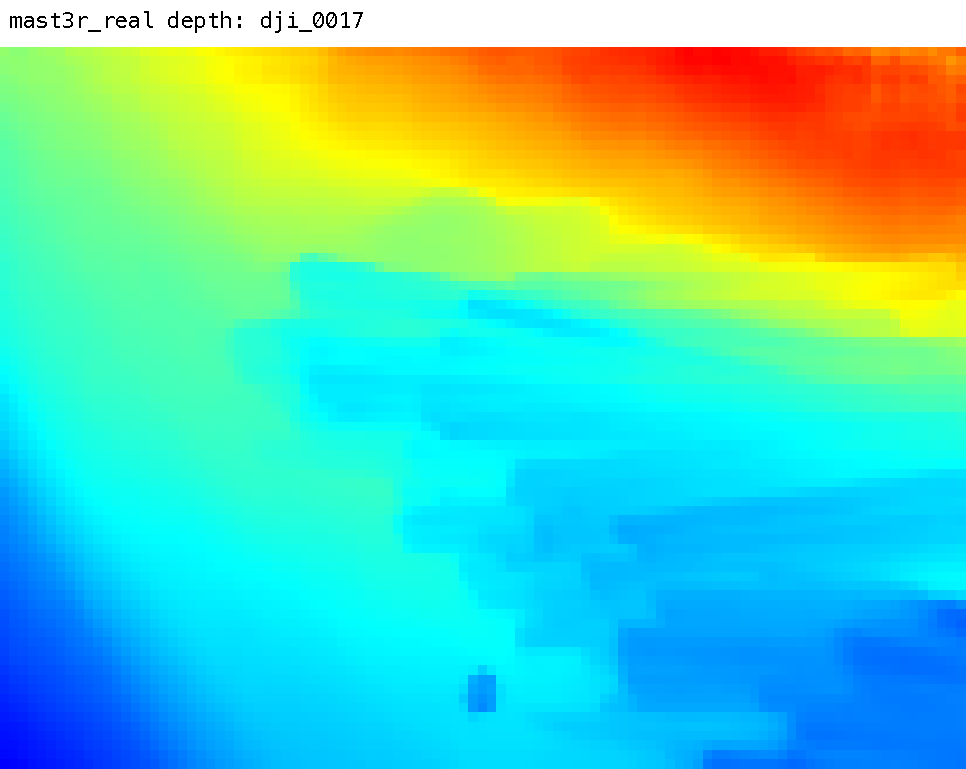
\includegraphics[width=\linewidth]{figures/odmdata_mast3r_depth.pdf}

\small (h) ODMData, MASt3R depth
\end{minipage}\hfill
\begin{minipage}[t]{0.31\linewidth}
\centering
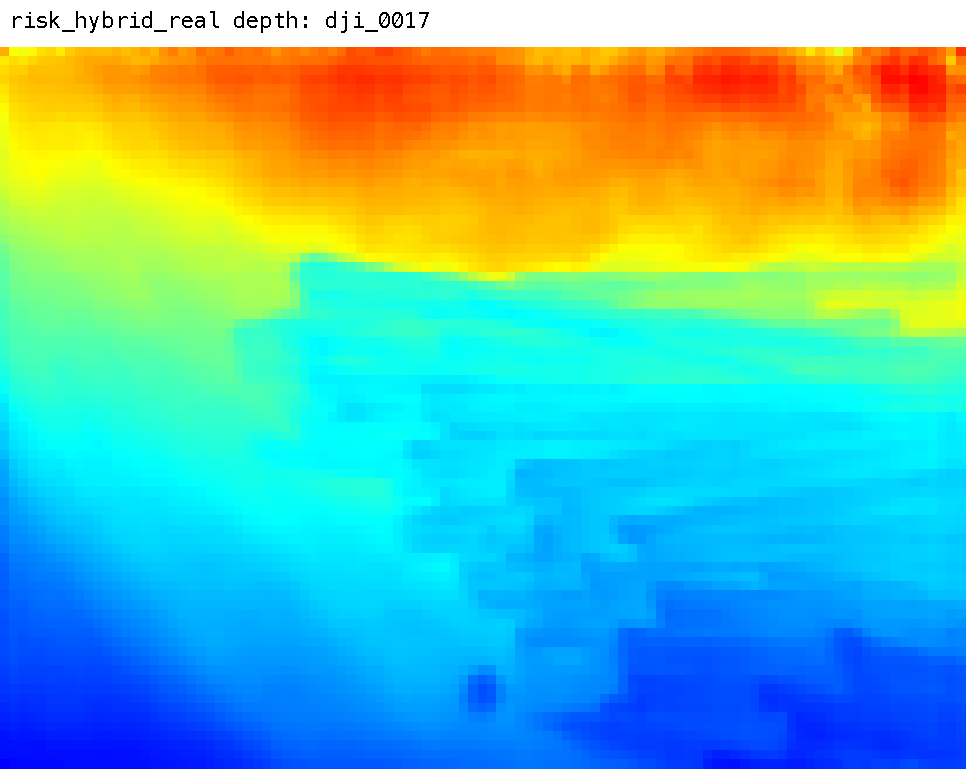
\includegraphics[width=\linewidth]{figures/odmdata_risk_depth.pdf}

\small (i) ODMData, risk-hybrid depth
\end{minipage}
\caption{Three-by-three qualitative comparison of the evaluated methods. The first row compares Dronescapes depth predictions, the second row compares Dronescapes error maps, and the third row compares ODMData depth predictions. Across both datasets, the proposed method visibly improves over the coarse DUSt3R baseline and remains close to the stronger MASt3R full-pass solution.}
\label{fig:qualitative-grid}
\end{figure}

\section{Discussion}

The primary strength of the current method is not best absolute accuracy, but \textbf{better use of refinement budget}. On both datasets, risk-hybrid narrows the gap between a coarse full-pass solution and a stronger full-pass solution while refining only a subset of frames. This is precisely the behavior the method was designed to induce.

At the same time, the present formulation has two clear limitations. First, it does not yet outperform full-pass MASt3R in absolute accuracy. Second, the risk score is still heuristic rather than learned, which means that it may miss more subtle uncertainty patterns that would be useful for frame selection.

The ODMData results also require careful interpretation because they are measured against projected depth maps derived from a saved COLMAP/OpenMVS reconstruction rather than direct geometric ground truth. They are useful for development and relative ranking, but they do not replace a metric geometry benchmark with direct ground truth.

Overall, the evidence supports risk-guided refinement as a \textbf{promising efficiency-oriented direction}, but not yet as a fully superior end-to-end reconstruction method.

\section{Conclusion}

This paper presented a selective-refinement strategy for UAV image-based geometry reconstruction. The proposed method combines a global DUSt3R coarse pass with MASt3R refinement on only the most risky frames. Experiments on Dronescapes and ODMData show that the method improves over DUSt3R on the ground-truth Dronescapes benchmark and stays competitive with DUSt3R on ODMData while refining only a fraction of frames.

However, the current implementation does not yet surpass MASt3R in absolute accuracy. The correct conclusion is therefore not that the proposed method is already the best solution, but that \textbf{risk-aware selective refinement is a credible and empirically supported direction for computation-aware UAV reconstruction}. The results justify further work on learned risk estimation, tighter integration between coarse and refined predictions, and more principled budget allocation schemes.

\bibliographystyle{elsarticle-num}
\bibliography{references}

\end{document}
